\begin{enumerate}
\item Find the distance between the following pairs of points:
\begin{enumerate}[label=(\roman*)]
\item $(2,3), (4,1)$
\item $(-5,7), (-1,3)$
\item $(a,b), (-a,b)$
\end{enumerate}
\item Find the distance between the points $(0,0)$ and $(36,15)$. Can you now find the two town A and B discussed in section $7.2$.
\item Determine if the points $(1,5), (2,3)$ and $(-2,11)$ are collinear.
\item Check whether $(5,2), (6,4)$ and $(7,2)$ are the vertices of an isoceles triangle.
\item In a classroom, $4$ friends are seated at the points $A, B, C$ and $D$ as shown \figref{fig:7.8} in  Champa and chameli walk into the class and  after observing for a fwe minutes champa asks chameli, \textquotedblleft Don't you think ABCD is a square?\textquotedblright  Chameli disagrees Using distance formula, find which of them is correct.
	\begin{figure}[ht]
\centering
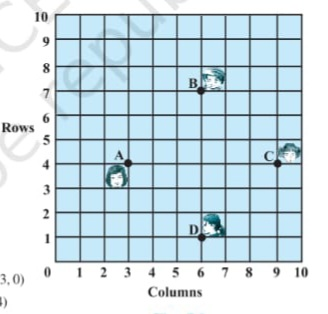
\includegraphics[width=\columnwidth]{chapters/10/figs/7.8.png}
\caption{7.8}
  \label{fig:7.8}
\end{figure}
\item Name the type of quadrilateral formed, if any, by the following points, and give reasons for your answer:
\begin{enumerate}[label=(\roman*)]
\item $(-1,2), (1,0), (-1,2), (3,0)$
\item $(-3,5), (3,1), (0,3), (-1,-4)$
\item $(4,5), (7,6), (4,3), (1,2)$
\end{enumerate}
\item Find the point on the $x$ axis which is equidistant from $(2,5)$ and $(2,9)$. 
\item Find the values of $y$ for which the distance between the points $P(2,-3)$ and $Q(10,y)$ is $10$ units.
\item $Q(0,1)$ is equidistant from $P(5,-3)$ and $R(x,6)$,find the values of $x$. Also find the distances $QR$ and $PR$.
\item Find a relation  between $x$ and $y$ such that $(x,y)$ is equidistant from the point $(3,6)$ and $(-3,4)$.
\end{enumerate}
	

